\chapter{Результаты экспериментов}
\label{chapter_results}

В данной главе приводятся результаты тестирования разработанных методов адаптивного выбора параметров ЭА на модельных задачах. Приводятся результаты сравнения существующих методов с существующими методами настройки параметров ЭА с помощью обучения с подкреплением. Также исследуется эффективность существующих методов выделения состояний среды.

\section{Описание экспериментов}

В качестве модельных задач используются известные задачи числовой оптимизации, а именно нахождение глобального минимума некоторой многомерной функции в ограниченной области с заданной точностью~$\epsilon$. Пусть $F(x_1, \ldots, x_n)$~-- оптимизируемая функция. При этом $x_i \in [min_i, max_i]$ для $1 \le i \le n$. В качестве функции приспособленности используется функция $F$. Поэтом более приспособленной считается особь с меньшим значением функции приспособленности.

В качестве особи ЭА, решающего заданную задачу, рассматривался набор из $n$ вещественных чисел. Пусть $x_1, \ldots, x_n$ -- текущее решение задачи оптимизации. В качестве эволюционных операторов применялся только оператор мутации, определяемый следующим образом:
\begin{equation}
x_i = \begin{cases}
	max_i, &\text{при } x_i + \sigma dx_i > max_i \\
	min_i, &\text{при } x_i + \sigma dx_i < min_i \\
	x_i + \sigma dx_i, &\text{иначе}
      \end{cases}, \text{для } 1 \le i \le n
\end{equation}
где $dx_i \sim \mathcal{N}(0, 1)$, а $\sigma$ -- настраиваемый параметр, называемый \textit{шагом}. Ожидаемым поведением методов адаптивного выбора параметров ЭА является уменьшение значения шага мутации при приближении к глобальному минимуму оптимизируемой функции. В проводимых экспериментах допустимые значения параметра $\sigma$ задаются интервалом $[0, k]$, где $k$ -- некоторая константа. В рамках данной работы проводились эксперименты с различными значениями параметра $k$. При увеличении параметра $k$ увеличивается диапазон допустимых значений параметра $\sigma$, что усложняет задачу поиска его оптимального значения.

В качестве ЭА, решающего поставленную задачу, используется $(\mu + \lambda)$ эволюционная стратегия. При увеличении $\lambda$ увеличивается число использований каждого выбранного значения параметра. Это способствует более точной оценке эффективности выбранного значения, однако сказывается на производительности. Кроме того, при тестировании предложенных и существующих методов настройки параметров ЭА нельзя ограничиться рассмотрением только $(1+\lambda)$ эволюционной стратегии. В самом деле, если в поколении всего одна особь, то из предложенных для построения дерева \textit{UTree} характеристик ЭА остается только число итераций без улучшения текущего решения. Таким образом, в рамках данной работы рассматривались различные значения параметра $\mu$, а в качестве характеристик ЭА использовались среднеквадратичное отклонение значений функции приспособленности в поколении, уменьшение среднего значения функции приспособленности и число итераций без улучшения текущего решения.

Пусть $f_t$~-- минимальное значение функции приспособленности на $t$-ом поколении ЭА. Награда вычисляется по формуле $R = c(\frac{f_t}{f_{t + 1}} - 1)$. При решении задачи минимизации при помощи $(\mu + \lambda)$ эволюционной стратегии, $f_{t + 1} \le f_t$. Поэтому агент всегда получает неотрицательную награду.

\subsection{Значения параметров}

В рамках проводимых экспериментов большинство параметров были взяты из статьи {karafotias}. В алгоритме $Q$-обучения были использованы следующие значения параметров:
\begin{itemize}
 \item $\alpha_0 = 0.2$~-- коэффициент скорости обучения при нулевой награде;
 \item $\alpha = 0.9$~-- коэффициент скорости обучения при положительной награде;
 \item $\gamma = 0.8$~-- дисконтный фактор;
 \item $\varepsilon = 0.1$~-- вероятность выбора случайного действия;
 \item $c = 100$~-- коэффициент масштабирования награды.
\end{itemize}

Эксперименты проводились для следующих значений парамеров ЭА:
\begin{itemize}
 \item $\mu \in \{1, 5, 10\}$~-- число особей в поколении;
 \item $\lambda \in \{1, 3, 7\}$~-- число потомков, создаваемых для каждой особи в процессе формирования следующего поколения;
 \item $\sigma \in \{1, 2, 3\}$~-- верхняя граница допустимых значений $\sigma$;
 \item $\epsilon = 10^{-5}$~-- допустимое отколонение решения от минимального значения оптимизируемой функции. 
\end{itemize}

\subsection{Описание результатов}

Введем следующие обозначения для исследуемых методов настройки параметров ЭА:
\begin{itemize}
 \item \textit{karafotias}~-- метод, предложенный \textit{Karafotias et al}.~(\ref{karafotias});
 \item \textit{q-learn}~-- метод настройки параметров ЭА с помощью $Q$-обучения с одним состоянием среды и множеством действий, заданным до начала работы алгоритма;
 \item \textit{earpc}~-- метод $earpc$~(\ref{earpc});
 \item \textit{uearpc}~-- метод на основе $earpc$ и $UTree$~(\ref{composing_method});
 \item \textit{adaptive}~-- метод с адаптивным выделением множества действий~(\ref{adaptive_method}).
\end{itemize}

Для каждого метода проводилось 50 запусков ЭА для каждой комбинации рассматриваемых значений параметров $k$, $\mu$, $\lambda$. Для каждой задачи было составлено три таблицы, в которых представлены усредненные по 50 запускам значения числа поколений, потребовавшихся для решения задачи, при различных значениях параметров ЭА. В первой из них находятся результаты работы метода \text{adaptive}. Остальные таблицы содержат сравнение пар методов \textit{karafotias} и \textit{q-learn}, \textit{earpc} и \textit{uearpc} при разных значениях $\mu$, $\sigma$ и $k$. Зеленым цветом выделяется лучшее значение среди всех исследуемых методов при заданных значениях параметров ЭА.
 
Далее подробно описываются модельные задачи, на которых проводилось экспериментальное исследование методов настройки параметров ЭА. Для каждой задачи приводятся результаты ее решения.
 
\section{Сфера}

Необходимо с точностью $\epsilon$ найти минимум унимодальной сферической функции~(\ref{sphere_eq}).
\begin{equation}
\label{sphere_eq}
f(x_1,..,x_n) = \sum\limits_{i=1}^n{x_i^2}
\end{equation}
График функции для двух переменных представлен на рис.~\ref{sphere_plot}. При $x_i \in [-10; 15]$ глобальный минимум достигается в точке $(0,..,0)$.

\begin{figure}
    \centering
    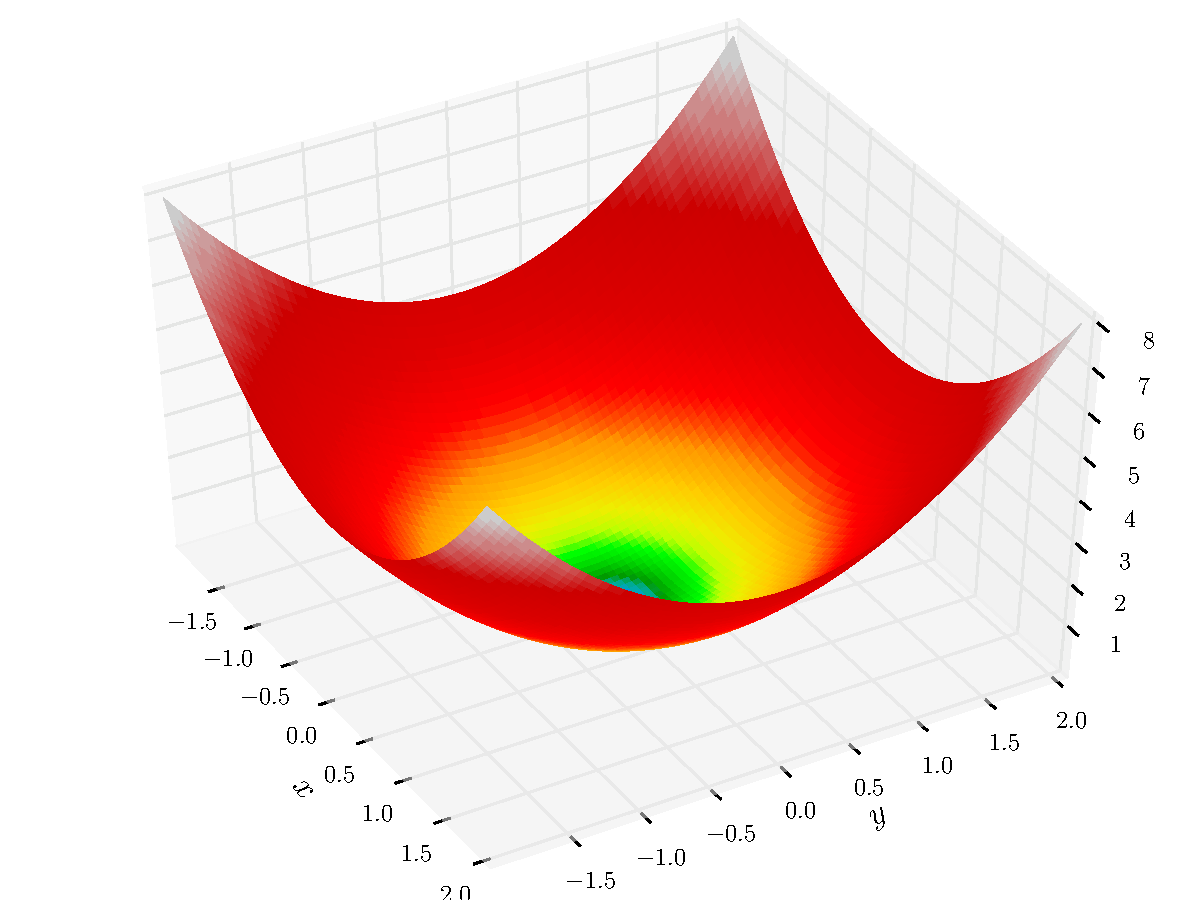
\includegraphics[width=0.6\textwidth]{sphere.pdf}
    \caption{График сферической функции для двух переменных.}
    \label{sphere_plot}
\end{figure}

Результаты применения исследуемых методов к данной задаче приведены в таблицах~\ref{adaptive_sphere_results}, \ref{q_sphere_results} и \ref{earpc_sphere_results}. Результаты подтверждают интуитивные предположения: для всех рассмотренных методов при увеличении параметров $\mu$ или $\lambda$, уменьшается среднее число поколений, потребовавшихся для нахождения минимума сферической функции, а при увеличении $k$ оно увеличивается. В самом деле, при увеличении параметров $\mu$ или $\lambda$ увеличивается число особей, рассматриваемых при формировании следующего поколения. Увеличение параметра $k$ увеличивает диапазон допустимых значений $\sigma$, что затрудняет выбор оптимального значения.

\begin{table}
  \centering
    \begin{tabular}{|*4{c|}}
    \hline
    \multicolumn{4}{|l|}{k = 1} \\
    \hline
    \diagbox{$\mu$}{$\lambda$} & \multicolumn{1}{c|}{1} & \multicolumn{1}{c|}{3} & \multicolumn{1}{c|}{7} \\
    \hline
    1 & \cellcolor{olive}{2434} & \cellcolor{olive}{2207}& \cellcolor{olive}{878} \\
    \hline
    5 & \cellcolor{olive}{1450} & \cellcolor{olive}{569} & \cellcolor{olive}{368} \\
    \hline
    10 & \cellcolor{olive}{703} & \cellcolor{olive}{331} & 186 \\
    \hline
    \multicolumn{4}{|l|}{k = 2} \\
    \hline
    \diagbox{$\mu$}{$\lambda$} & \multicolumn{1}{c|}{1} & \multicolumn{1}{c|}{3} & \multicolumn{1}{c|}{7} \\
    \hline
    1 & \cellcolor{olive}{4342}& \cellcolor{olive}{2333}& \cellcolor{olive}{1464} \\
    \hline
    5 & \cellcolor{olive}{1891} & 974& \cellcolor{olive}{616} \\
    \hline
    10 & 1164 & 459& \cellcolor{olive}{188} \\
    \hline
    \multicolumn{4}{|l|}{k = 3} \\
    \hline
    \diagbox{$\mu$}{$\lambda$} & \multicolumn{1}{c|}{1} & \multicolumn{1}{c|}{3} & \multicolumn{1}{c|}{7} \\
    \hline
    1 & \cellcolor{olive}{8055}& \cellcolor{olive}{2826}& \cellcolor{olive}{1427} \\
    \hline
    5 & \cellcolor{olive}{2447} & 1445 & 896 \\
    \hline
    10 & \cellcolor{olive}{1996}& \cellcolor{olive}{1053} & 409 \\
  \hline
  \end{tabular}
  \captionsetup{justification=centering}
  \caption{Таблица с результатами применения метода \text{adaptive} для сферической функции.}
  \label{adaptive_sphere_results}
\end{table}

\begin{table}
  \centering
  \begin{tabular}{|*7{c|}}
    \hline
    \multicolumn{7}{|l|}{k = 1} \\
    \hline
    \multirow{2}{*}{\diagbox{$\mu$}{$\lambda$}} & \multicolumn{2}{c|}{1} & \multicolumn{2}{c|}{3} & \multicolumn{2}{c|}{7} \\
    \cline{2-7}
    & q-learn & karafotias & q-learn & karafotias & q-learn & karafotias \\
    \hline
    1 & 8769 & 8048 & 4221 & 2683 & 1085 & 2620 \\
    \hline
    5 & 1664 & 2076 & 706 & 824 & 390 & 473 \\
    \hline
    10 & 959& 747 & 378 & 358 & 195 & \cellcolor{olive}{167} \\
    \hline
    \multicolumn{7}{|l|}{k = 2} \\
    \hline
    \multirow{2}{*}{\diagbox{$\mu$}{$\lambda$}} & \multicolumn{2}{c|}{1} & \multicolumn{2}{c|}{3} & \multicolumn{2}{c|}{7} \\
    \cline{2-7}
    & q-learn & karafotias & q-learn & karafotias & q-learn & karafotias \\
    \hline
    1 & 25192 & 28523 & 7681 & 6478 & 3360 & 3739 \\
    \hline
    5 & 3814 & 3468 & 994 & 1163 & 716 & 756 \\
    \hline
    10 & 2397 & 1833& \cellcolor{olive}{445} & 465 & 320 & 252 \\
    \hline
    \multicolumn{7}{|l|}{k = 3} \\
    \hline
    \multirow{2}{*}{\diagbox{$\mu$}{$\lambda$}} & \multicolumn{2}{c|}{1} & \multicolumn{2}{c|}{3} & \multicolumn{2}{c|}{7} \\
    \cline{2-7}
    & q-learn & karafotias & q-learn & karafotias & q-learn & karafotias \\
    \hline
    1 & 36698 & 29112 & 7845 & 9115 & 3907 & 4813 \\
    \hline
    5 & 8328 & 5886 & 2790 & 2222 & 919 & \cellcolor{olive}{777} \\
    \hline
    10 & 2398 & 2531 & 1074 & 1206& \cellcolor{olive}{391} & 427 \\
    \hline
    \end{tabular}
  \captionsetup{justification=centering}
  \caption{Таблица с результатами применения методов \text{q-learn} и \text{karafotias} для сферической функции.}
  \label{q_sphere_results}
\end{table}

\begin{table}
  \centering
  \begin{tabular}{|*7{c|}}
    \hline
    \multicolumn{7}{|l|}{k = 1} \\
    \hline
    \multirow{2}{*}{\diagbox{$\mu$}{$\lambda$}} & \multicolumn{2}{c|}{1} & \multicolumn{2}{c|}{3} & \multicolumn{2}{c|}{7} \\
    \cline{2-7}
    & earpc & uearpc & earpc & uearpc & earpc & uearpc \\
    \hline
    1 & 5258 & 4830 & 3942 & 3070 & 1653 & 2247 \\
    \hline
    5 & 4472 & 3893 & 1589 & 845 & 642& 568 \\
    \hline
    10 & 1438 & 728 & 534 & 400& 142 & 422 \\
    \hline
    \multicolumn{7}{|l|}{k = 2} \\
    \hline
    \multirow{2}{*}{\diagbox{$\mu$}{$\lambda$}} & \multicolumn{2}{c|}{1} & \multicolumn{2}{c|}{3} & \multicolumn{2}{c|}{7} \\
    \cline{2-7}
    & earpc & uearpc & earpc & uearpc & earpc & uearpc \\
    \hline
    1 & 31738 & 16182 & 5152 & 4233 & 1688 & 2956 \\
    \hline
    5 & 4908 & 5173 & 1631& \cellcolor{olive}{946} & 1511 & 626 \\
    \hline
    10& \cellcolor{olive}{778} & 876 & 719 & 788 & 380 & 413 \\
    \hline
    \multicolumn{7}{|l|}{k = 3} \\
    \hline
    \multirow{2}{*}{\diagbox{$\mu$}{$\lambda$}} & \multicolumn{2}{c|}{1} & \multicolumn{2}{c|}{3} & \multicolumn{2}{c|}{7} \\
    \cline{2-7}
    & earpc & uearpc & earpc & uearpc & earpc & uearpc \\
    \hline
    1 & 54868 & 30710 & 12446 & 11985 & 10118 & 9207 \\
    \hline
    5 & 3348 & 12313& \cellcolor{olive}{1379} & 1848 & 1424 & 1105 \\
    \hline
    10 & 3173 & 3745 & 1114 & 1712 & 410 & 537 \\
    \hline
  \end{tabular}
  \captionsetup{justification=centering}
  \caption{Таблица с результатами применения методов \text{earpc} и \text{uearpc} для сферической функции.}
  \label{earpc_sphere_results}
\end{table}

Предложенный метод \textit{adaptive} превосходит остальные рассматриваемые методы на большинстве конфигураций ЭА. Отметим, что при значении параметра $\mu$ равном единице, то есть в случае когда поколение состоит из одной особи, число итераций ЭА, понадобившихся для решения задачи, с помощью метода \textit{adaptive} оказалось в разы меньше, чем при использовании остальных методов. Это можно объяснить тем, что в методе предложенном \textit{Karafotias et al}. награда, полученная за использование того или иного значения параметра, перестает учитываться со временем работы алгоритма. В методе \textit{adaptive} отсутствует данный недостаток, так как полученный опыт сохраняется не только в значениях ожидаемой награды, но и в разбиении диапазона значений оптимизируемого параметра. Это происходит в случае продолжительного выбора неэффективного значения параметра. В методе \textit{uearpc} разбиение диапазона значений настраеваемого параметра происходит на основе кластеризации значений и при этом не учитываются значения награды. Данные предположения подтверждаются графиками распределения выбранных значений параметра $\sigma$ в предложенных методах, приведенными на рис.~\ref{uarpc_sphere_plot}, \ref{adaptive_sphere_plot} и \ref{karafotias_sphere}.

На графике~\ref{uarpc_sphere_plot} видно, что в конце работы алгоритма \textit{uearpc} значения настраеваемого параметра $\sigma$ выбираются случайно из всего диапазона допустимых значений. При этом диапазон разбивается на два интервала почти равного размера. На графике~\ref{karafotias_sphere} видно, что при получении положительной награды за подбор эффективного значения параметра алгоритм~\textit{karafotias} продолжает выбирать значения параметра из того же интервала. Но если на протяжении нескольких итераций не была получена положительная награда, алгоритм теряет информацию о ранее выбранном эффективном значении. На графике~\ref{adaptive_sphere_plot} видно, что на протяжении всего процесса оптимизации алгоритм \textit{adaptive} приближает значение настраеваемого параметра к оптимальному. При этом в начале работы алгоритма в течение некоторого числа итераций значения выбираются случайным образом, так как полученного опыта недостаточно для разбиения диапазона значений. В ходе работы пересчитываются размеры интервалов разбиения. А в конце работы алгоритм уменьшает необходимое число интервалов.

Отметим, что при применении методов \textit{karafotias} и \textit{q-learn}, \textit{earpc} и \textit{uearpc} были получены схожие результаты. Таким образом, выделение состояний среды слабо влияет на эффективность настройки значений параметров.

\begin{figure}
  \centering
  \subfloat[График выбранных значений $\sigma$.]{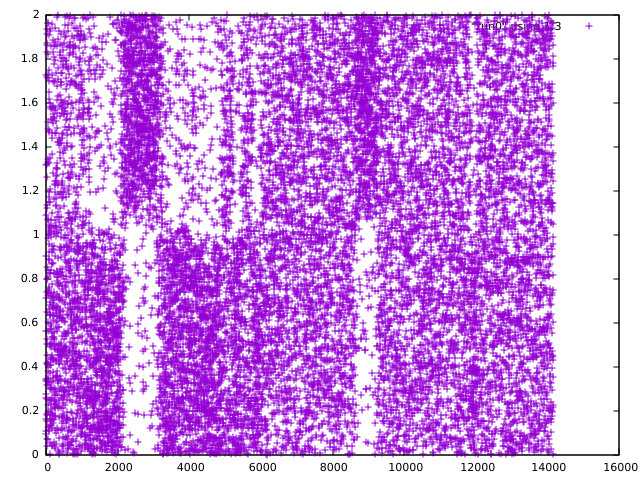
\includegraphics[width=0.5\textwidth]{earpc_sphere_dist.png}}
  \subfloat[График значения точки разбиения.]{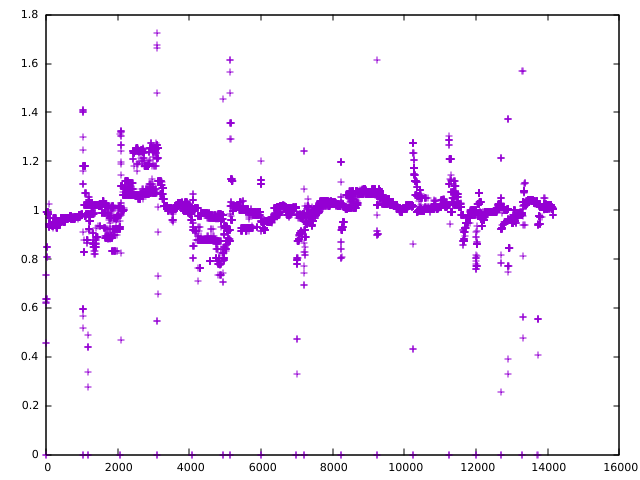
\includegraphics[width=0.5\textwidth]{earpc_sphere.png}}
  \caption{ Графики работы метода \textit{uarpc} для сферической функции.}
  \label{uarpc_sphere_plot}
\end{figure}

\begin{figure}
  \centering
  \subfloat[График выбранных значений $\sigma$.]{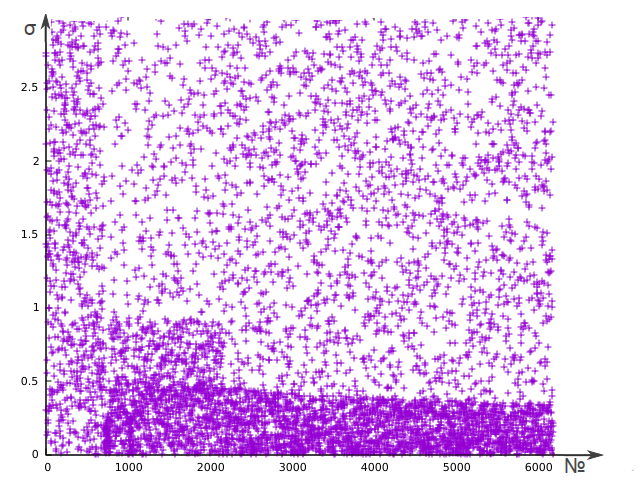
\includegraphics[width=0.5\textwidth]{adaptive_sphere_dist.png}}
  \subfloat[График значения точек разбиения.]{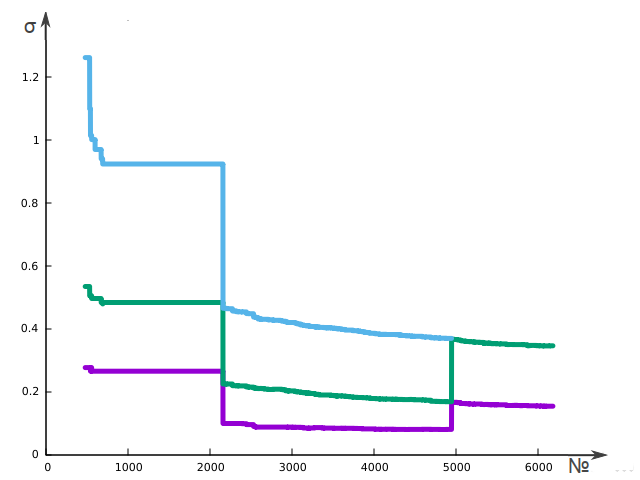
\includegraphics[width=0.5\textwidth]{adaptive_sphere.png}}
  \caption{ Графики работы метода \textit{adaptive} для сферической функции.}
  \label{adaptive_sphere_plot}
\end{figure}

\begin{figure}
  \centering
  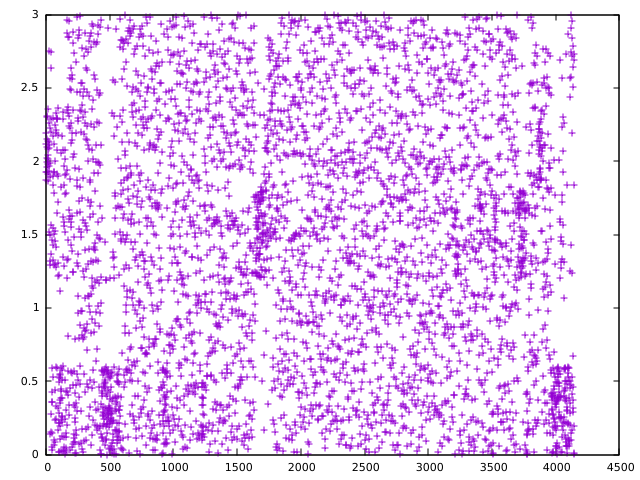
\includegraphics[width=0.5\textwidth]{karafotias_sphere.png}
  \caption{График выбранных значений $\sigma$ в методе \textit{karafotias} для сферической функции.}
  \label{karafotias_sphere}
\end{figure}


\section{Функция Розенброка}

Предложенная Ховардом Розенброком невыпуклая функция~(\ref{rosenbrock_eq}) часто используется для оценки производительности алгоритмов оптимизации. Обычно в качестве значений $a$ и $b$ выбираются $a = 1$, $b = 100$. График функции для двух переменных представлен на рис.~\ref{rosenbrock_plot}. Считается, что поиск глобального минимума данной функции при помощи алгоритмов оптимизации является нетривиальной задачей. Это объясняется тем, что глобальный минимум находится в длинной, узкой \textit{впадине}, найти которую обычно не составляет труда. Трудность заключается в поиске минимума в этой впадине. При $x_i \in [-15; 10]$ он достигается в точке $(1,..,1)$.

\begin{equation}
\label{rosenbrock_eq}
f(x_1, x_2) = (a - x_1^2)^2 + b(x_2 - x_1^2)^2
\end{equation}


\begin{figure}
    \centering
    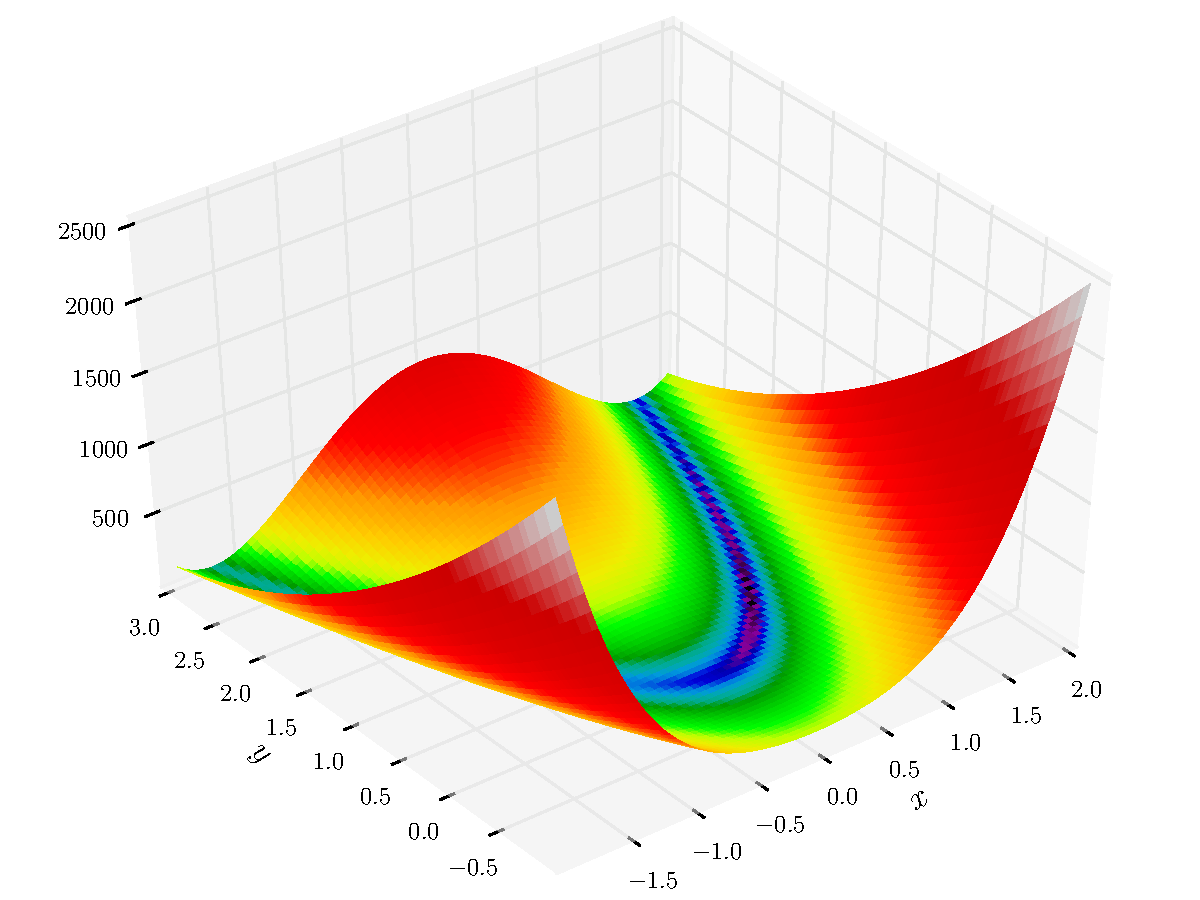
\includegraphics[width=0.6\textwidth]{rosenbrock.pdf}
    \caption{График функции Розенброка для двух переменных.}
    \label{rosenbrock_plot}
\end{figure}

\begin{table}
  \centering
  \begin{tabular}{|*4{c|}}
    \hline
    \multicolumn{4}{|l|}{k = 1} \\
    \hline
    \diagbox{$\mu$}{$\lambda$} & \multicolumn{1}{c|}{1} & \multicolumn{1}{c|}{3} & \multicolumn{1}{c|}{7} \\
    \hline
    1 & \cellcolor{olive}{3631} & \cellcolor{olive}{1776} & \cellcolor{olive}{1226} \\
    \hline
    5 & \cellcolor{olive}{1666} & 918& \cellcolor{olive}{502} \\
    \hline
    10 & \cellcolor{olive}{1008} & 622& \cellcolor{olive}{358} \\
    \hline
    \multicolumn{4}{|l|}{k = 2} \\
    \hline
    \diagbox{$\mu$}{$\lambda$} & \multicolumn{1}{c|}{1} & \multicolumn{1}{c|}{3} & \multicolumn{1}{c|}{7} \\
    \hline
    1 & \cellcolor{olive}{4744}& \cellcolor{olive}{1839}& \cellcolor{olive}{1160} \\
    \hline
    5 & \cellcolor{olive}{2467}& \cellcolor{olive}{1128} & 967 \\
    \hline
    10 & \cellcolor{olive}{1722}& \cellcolor{olive}{988}& \cellcolor{olive}{615} \\
    \hline
    \multicolumn{4}{|l|}{k = 3} \\
    \hline
    \diagbox{$\mu$}{$\lambda$} & \multicolumn{1}{c|}{1} & \multicolumn{1}{c|}{3} & \multicolumn{1}{c|}{7} \\
    \hline
    1 & \cellcolor{olive}{5159}& \cellcolor{olive}{2821} & \cellcolor{olive}{1517} \\
    \hline
    5 & \cellcolor{olive}{2704} & \cellcolor{olive}{1544} & \cellcolor{olive}{902} \\
    \hline
    10 & \cellcolor{olive}{2048} & 1296 & 955 \\
  \hline
  \end{tabular}
  \captionsetup{justification=centering}
  \caption{Таблица с результатами применения метода \text{adaptive} для функции Розенброка.}
\end{table}

\begin{table}
\centering
  \begin{tabular}{|*7{c|}}
    \hline
    \multicolumn{7}{|l|}{k = 1} \\
    \hline
    \multirow{2}{*}{\diagbox{$\mu$}{$\lambda$}} & \multicolumn{2}{c|}{1} & \multicolumn{2}{c|}{3} & \multicolumn{2}{c|}{7} \\
    \cline{2-7}
    & q-learn & karafotias & q-learn & karafotias & q-learn & karafotias \\
    \hline
    1 & 9653 & 8385 & 2226& 2069& 1605 & 1757 \\
    \hline
    5 & 1706 & 2281& \cellcolor{olive}{894} & 942 & 570 & 675 \\
    \hline
    10 & 1103 & 1105& \cellcolor{olive}{604} & 665 & 489 & 473 \\
    \hline
    \multicolumn{7}{|l|}{k = 2} \\
    \hline
    \multirow{2}{*}{\diagbox{$\mu$}{$\lambda$}} & \multicolumn{2}{c|}{1} & \multicolumn{2}{c|}{3} & \multicolumn{2}{c|}{7} \\
    \cline{2-7}
    & q-learn & karafotias & q-learn & karafotias & q-learn & karafotias \\
    \hline
    1 & 23663 & 21043 & 6405 & 6825 & 2388 & 2183 \\
    \hline
    5 & 3944 & 4029 & 1614 & 1780 & 1012 & 1461 \\
    \hline
    10 & 2108 & 2255 & 1420 & 1116 & 856 & 712 \\
    \hline
    \multicolumn{7}{|l|}{k = 3} \\
    \hline
    \multirow{2}{*}{\diagbox{$\mu$}{$\lambda$}} & \multicolumn{2}{c|}{1} & \multicolumn{2}{c|}{3} & \multicolumn{2}{c|}{7} \\
    \cline{2-7}
    & q-learn & karafotias & q-learn & karafotias & q-learn & karafotias \\
    \hline
    1 & 29082 & 23305 & 7977 & 10726 & 4680 & 4266 \\
    \hline
    5 & 6208 & 5419 & 2514 & 2096 & 1120 & 1629 \\
    \hline
    10 & 3747 & 3258 & 1740 & 1523 & 995 & 1203 \\
    \hline
  \end{tabular}
  \captionsetup{justification=centering}
  \caption{Таблица с результатами применения методов \text{q-learn} и \text{karafotias} для функции Розенброка.}
\end{table}

\begin{table}
  \centering
  \begin{tabular}{|*7{c|}}
    \hline
    \multicolumn{7}{|l|}{k = 1} \\
    \hline
    \multirow{2}{*}{\diagbox{$\mu$}{$\lambda$}} & \multicolumn{2}{c|}{1} & \multicolumn{2}{c|}{3} & \multicolumn{2}{c|}{7} \\
    \cline{2-7}
    & earpc & uearpc & earpc & uearpc & earpc & uearpc \\
    \hline
    1 & 7794 & 8689 & 3148 & 3610 & 1422 & 1422 \\
    \hline
    5 & 4341 & 4530 & 1958 & 2197 & 1679 & 1329 \\
    \hline
    10 & 2681 & 2926 & 1460 & 1485 & 1103 & 1858 \\
    \hline
    \multicolumn{7}{|l|}{k = 2} \\
    \hline
    \multirow{2}{*}{\diagbox{$\mu$}{$\lambda$}} & \multicolumn{2}{c|}{1} & \multicolumn{2}{c|}{3} & \multicolumn{2}{c|}{7} \\
    \cline{2-7}
    & earpc & uearpc & earpc & uearpc & earpc & uearpc \\
    \hline
    1 & 27865 & 19142 & 9748 & 8997 & 3806 & 4085 \\
    \hline
    5 & 5961 & 5750 & 2293 & 1720& \cellcolor{olive}{933} & 1180 \\
    \hline
    10 & 2411 & 2807 & 1486 & 1234 & 627 & 922 \\
    \hline
    \multicolumn{7}{|l|}{k = 3} \\
    \hline
    \multirow{2}{*}{\diagbox{$\mu$}{$\lambda$}} & \multicolumn{2}{c|}{1} & \multicolumn{2}{c|}{3} & \multicolumn{2}{c|}{7} \\
    \cline{2-7}
    & earpc & uearpc & earpc & uearpc & earpc & uearpc \\
    \hline
    1 & 24249 & 27327 & 6541 & 16040 & 4144 & 5408 \\
    \hline
    5 & 5953 & 7665 & 2823& 2304 & 1033 & 1055 \\
    \hline
    10 & 5095 & 3873& \cellcolor{olive}{1013} & 1028& \cellcolor{olive}{779} & 839 \\
    \hline
  \end{tabular}
  \captionsetup{justification=centering}
  \caption{Таблица с результатами применения методов \text{earpc} и \text{uearpc} для функции Розенброка.}
\end{table}

\begin{figure}
  \centering
  \subfloat[График выбранных значений $\sigma$.]{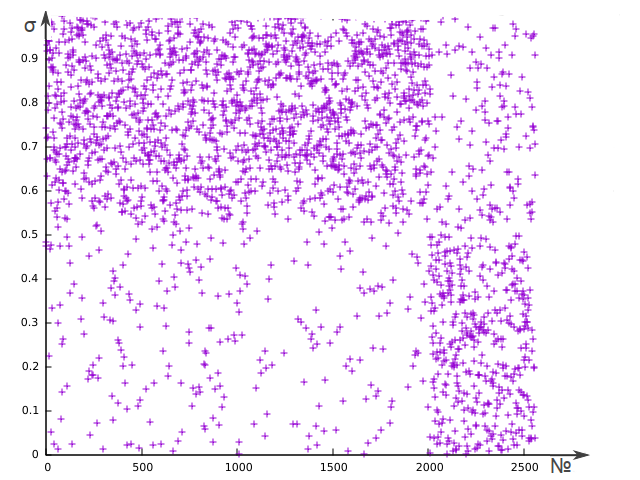
\includegraphics[width=0.5\textwidth]{earpc_rosenbrock_dist.png}}
  \subfloat[График значения точки разбиения.]{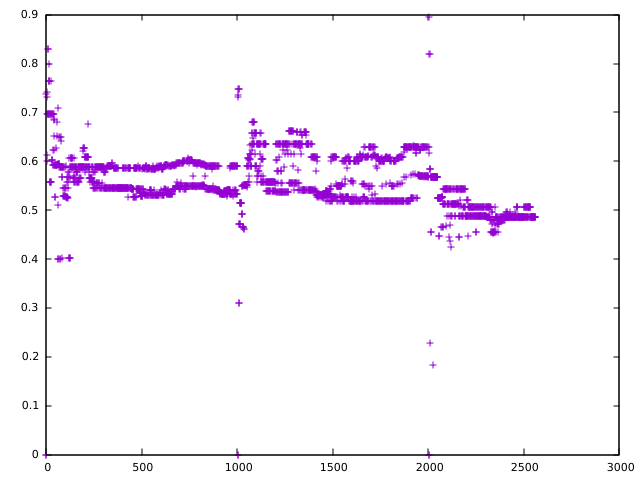
\includegraphics[width=0.5\textwidth]{earpc_rosenbrock.png}}
  \caption{ Графики работы метода \textit{uarpc} для функции Розенброка.}
  \label{uarpc_rosenbrock_plot}
\end{figure}

\begin{figure}
  \centering
  \subfloat[График выбранных значений $\sigma$.]{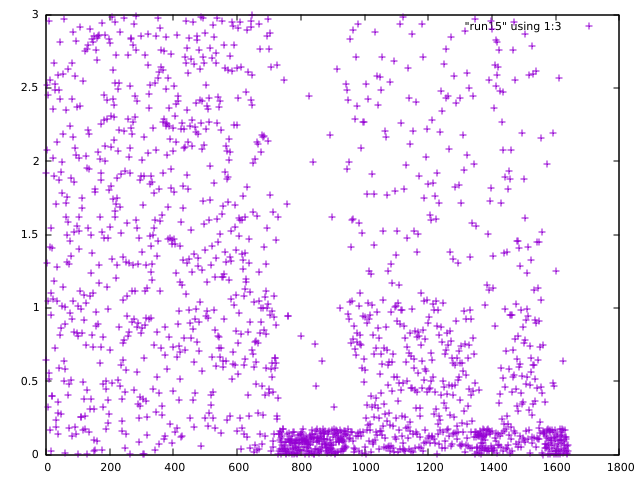
\includegraphics[width=0.5\textwidth]{adaptive_rosenbrock_dist.png}}
  \subfloat[График значения точек разбиения.]{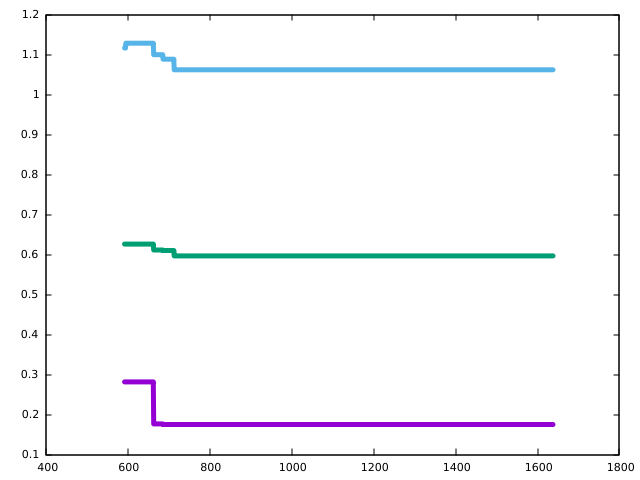
\includegraphics[width=0.5\textwidth]{adaptive_rosenbrock.png}}
  \caption{ Графики работы метода \textit{adaptive} для функции Розенброка.}
  \label{adaptive_rosenbrock_plot}
\end{figure}

\begin{figure}
  \centering
  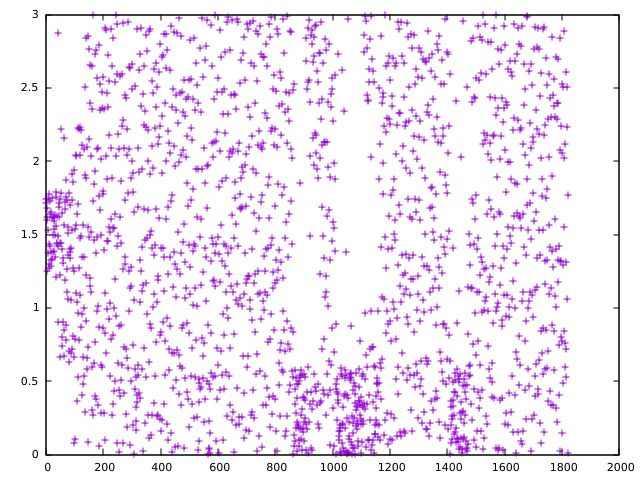
\includegraphics[width=0.5\textwidth]{karafotias_rosenbrock.png}
  \caption{График выбранных значений $\sigma$ в методе \textit{karafotias} для функции Розенброка.}
  \label{karafotias_rosenbrock}
\end{figure}

\section{Функция Леви}

Мультимодальная функция Леви для двух переменных задается формулой~(\ref{levi_eq}). График функции представлен на рис.~\ref{levi_plot}. При $x, y \in [-10; 10]$ минимум достигается в точке $(1, 1)$.

\begin{equation}
\label{levi_eq}
\begin{split}
f(x_1, x2) = &sin^2(3\pi x) + (x - 1)^2(1 + sin^2(3\pi y)) + \\
& + (y - 1)^2(1 + sin^2(2\pi y))
\end{split}
\end{equation}

\begin{figure}
    \centering
    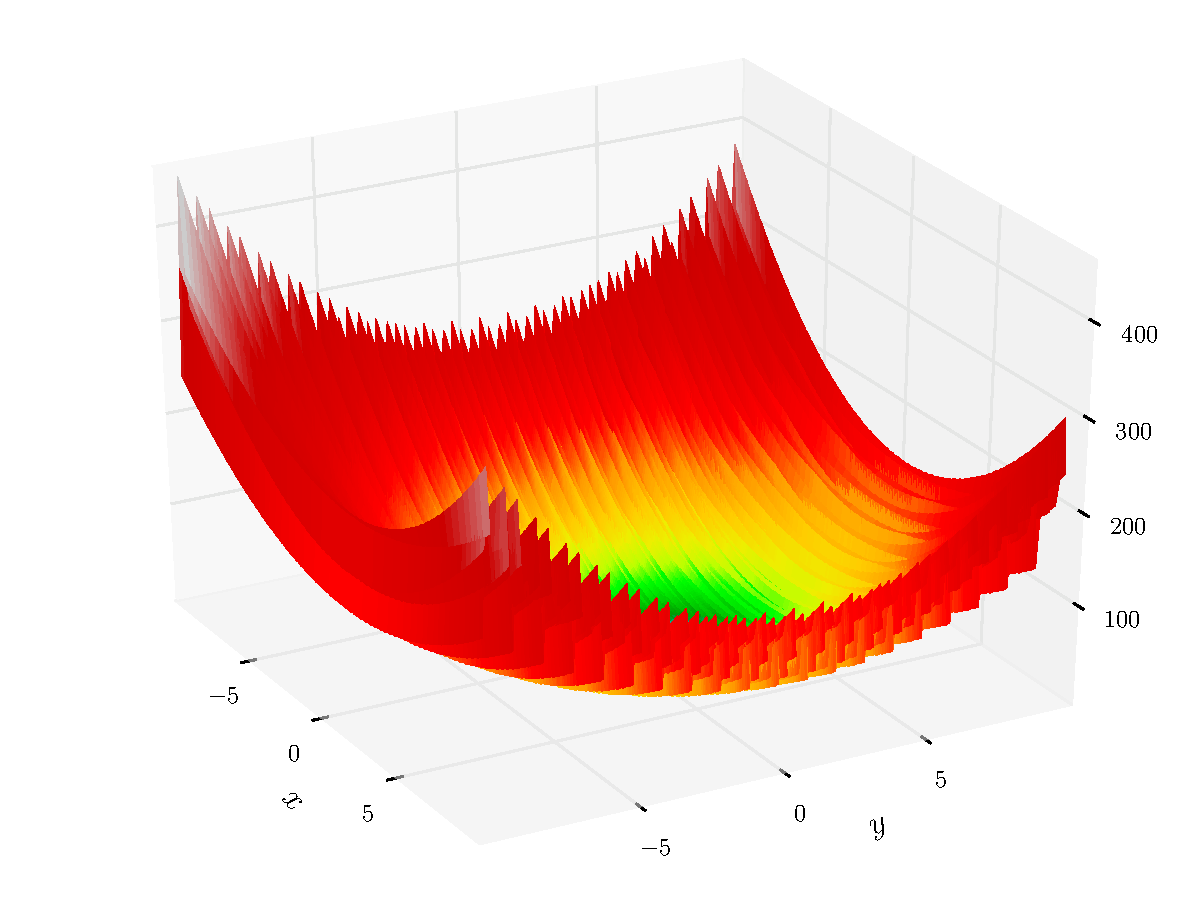
\includegraphics[width=0.6\textwidth]{levi.pdf}
    \caption{График функции Леви для двух переменных.}
    \label{levi_plot}
\end{figure}

\begin{table}
  \centering
  \begin{tabular}{|*4{c|}}
    \hline
    \multicolumn{4}{|l|}{k = 1} \\
    \hline
    \diagbox{$\mu$}{$\lambda$} & \multicolumn{1}{c|}{1} & \multicolumn{1}{c|}{3} & \multicolumn{1}{c|}{7} \\
    \hline
    1& \cellcolor{olive}{3496} & \cellcolor{olive}{1980} & \cellcolor{olive}{1321} \\
    \hline
    5& \cellcolor{olive}{1778} & 855 & \cellcolor{olive}{356} \\
    \hline
    10 & 884 & 533 & 308 \\
    \hline
    \multicolumn{4}{|l|}{k = 2} \\
    \hline
    \diagbox{$\mu$}{$\lambda$} & \multicolumn{1}{c|}{1} & \multicolumn{1}{c|}{3} & \multicolumn{1}{c|}{7} \\
    \hline
    1 & \cellcolor{olive}{4947} & \cellcolor{olive}{2020} & \cellcolor{olive}{1205} \\
    \hline
    5 & \cellcolor{olive}{1935} & \cellcolor{olive}{1085} & \cellcolor{olive}{770} \\
    \hline
    10 & \cellcolor{olive}{1803} & \cellcolor{olive}{887} & 618 \\
    \hline
    \multicolumn{4}{|l|}{k = 3} \\
    \hline
    \diagbox{$\mu$}{$\lambda$} & \multicolumn{1}{c|}{1} & \multicolumn{1}{c|}{3} & \multicolumn{1}{c|}{7} \\
    \hline
    1 & \cellcolor{olive}{5216}& \cellcolor{olive}{2900} & \cellcolor{olive}{1700} \\
    \hline
    5 & \cellcolor{olive}{3105} & \cellcolor{olive}{1808} & 1017 \\
    \hline
    10 & \cellcolor{olive}{2071}& \cellcolor{olive}{1330} & 667 \\
    \hline
  \end{tabular}
  \captionsetup{justification=centering}
  \caption{Таблица с результатами применения метода \text{adaptive} для функции Леви.}
\end{table}

\begin{table}
  \centering
  \begin{tabular}{|*7{c|}}
  \hline
  \multicolumn{7}{|l|}{k = 1} \\
  \hline
  \multirow{2}{*}{\diagbox{$\mu$}{$\lambda$}} & \multicolumn{2}{c|}{1} & \multicolumn{2}{c|}{3} & \multicolumn{2}{c|}{7} \\
  \cline{2-7}
  & q-learn & karafotias & q-learn & karafotias & q-learn & karafotias \\
  \hline
  1 & 7200 & 7265 & 3305 & 2903 & 1584 & 1600 \\
  \hline
  5 & 1898 & 1865 & 862 & \cellcolor{olive}{794} & 606 & 444 \\
  \hline
  10 & 840& \cellcolor{olive}{804} & \cellcolor{olive}{502} & 624 & 331 & \cellcolor{olive}{294} \\
  \hline
  \multicolumn{7}{|l|}{k = 2} \\
  \hline
  \multirow{2}{*}{\diagbox{$\mu$}{$\lambda$}} & \multicolumn{2}{c|}{1} & \multicolumn{2}{c|}{3} & \multicolumn{2}{c|}{7} \\
  \cline{2-7}
  & q-learn & karafotias & q-learn & karafotias & q-learn & karafotias \\
  \hline
  1 & 13420 & 14789 & 6884 & 6601 & 3521 & 2370 \\
  \hline
  5 & 3517 & 3369 & 1231 & 1326 & 792 & 1089 \\
  \hline
  10 & 1884 & 2197 & 988 & 1006 & 731& \cellcolor{olive}{564} \\
  \hline
  \multicolumn{7}{|l|}{k = 3} \\
  \hline
  \multirow{2}{*}{\diagbox{$\mu$}{$\lambda$}} & \multicolumn{2}{c|}{1} & \multicolumn{2}{c|}{3} & \multicolumn{2}{c|}{7} \\
  \cline{2-7}
  & q-learn & karafotias & q-learn & karafotias & q-learn & karafotias \\
  \hline
  1 & 21470 & 21953 & 9029 & 7071 & 4139 & 4019 \\
  \hline
  5 & 6966 & 6742& 2467 & 2664 & 1929 & 1788 \\
  \hline
  10 & 2901 & 2943 & 1462 & 1832 & 1117 & 799 \\
  \hline
  \end{tabular}
  \captionsetup{justification=centering}
  \caption{Таблица с результатами применения методов \text{q-learn} и \text{karafotias} для функции Леви.}
\end{table}

\begin{table}
  \centering
  \begin{tabular}{|*7{c|}}
    \hline
    \multicolumn{7}{|l|}{k = 1} \\
    \hline
    \multirow{2}{*}{\diagbox{$\mu$}{$\lambda$}} & \multicolumn{2}{c|}{1} & \multicolumn{2}{c|}{3} & \multicolumn{2}{c|}{7} \\
    \cline{2-7}
    & earpc & uearpc & earpc & uearpc & earpc & uearpc \\
    \hline
    1 & 7986 & 14092 & 2789 & 3688 & 1923 & 3820 \\
    \hline
    5 & 2372 & 2246 & 1632 & 2171 & 1426 & 1236 \\
    \hline
    10 & 2353 & 1451 & 1491 & 1134 & 510 & 766 \\
    \hline
    \multicolumn{7}{|l|}{k = 2} \\
    \hline
    \multirow{2}{*}{\diagbox{$\mu$}{$\lambda$}} & \multicolumn{2}{c|}{1} & \multicolumn{2}{c|}{3} & \multicolumn{2}{c|}{7} \\
    \cline{2-7}
    & earpc & uearpc & earpc & uearpc & earpc & uearpc \\
    \hline
    1 & 25721 & 30653 & 7477 & 4612 & 2533 & 2967 \\
    \hline
    5 & 7222 & 5365 & 3039 & 2943 & 1153 & 2180 \\
    \hline
    10 & 5139 & 3072 & 1045 & 2381 & 806 & 1064 \\
    \hline
    \multicolumn{7}{|l|}{k = 3} \\
    \hline
    \multirow{2}{*}{\diagbox{$\mu$}{$\lambda$}} & \multicolumn{2}{c|}{1} & \multicolumn{2}{c|}{3} & \multicolumn{2}{c|}{7} \\
    \cline{2-7}
    & earpc & uearpc & earpc & uearpc & earpc & uearpc \\
    \hline
    1 & 28900 & 35119 & 6966 & 10883 & 3375 & 2062 \\
    \hline
    5 & 10480 & 9059 & 4593 & 3714 & \cellcolor{olive}{594} & 1439 \\
    \hline
    10 & 5210 & 4814 & 3140 & 2389 & \cellcolor{olive}{521} & 845 \\
    \hline
  \end{tabular}
  \captionsetup{justification=centering}
  \caption{Таблица с результатами применения методов \text{earpc} и \text{uearpc} для функции Леви.}
\end{table}

\begin{figure}
  \centering
  \subfloat[График выбранных значений $\sigma$.]{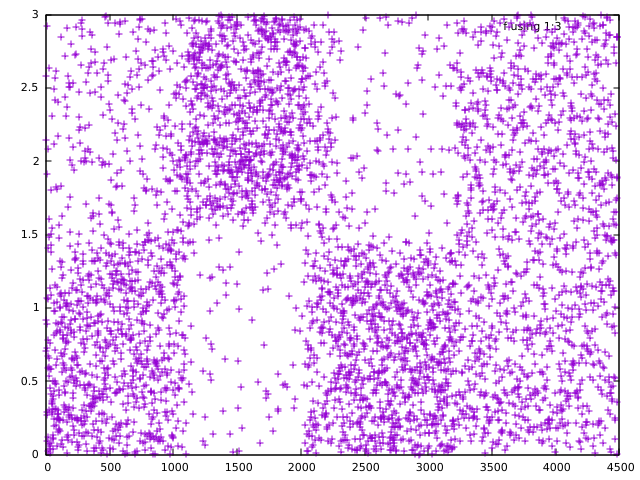
\includegraphics[width=0.5\textwidth]{earpc_levi_dist.png}}
  \subfloat[График значения точки разбиения.]{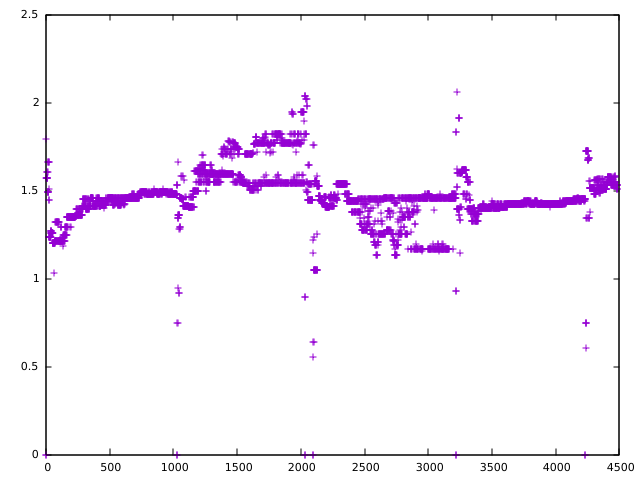
\includegraphics[width=0.5\textwidth]{earpc_levi.png}}
  \caption{ Графики работы метода \textit{uarpc} для функции Леви.}
  \label{uarpc_levi_plot}
\end{figure}

\begin{figure}
  \centering
  \subfloat[График выбранных значений $\sigma$.]{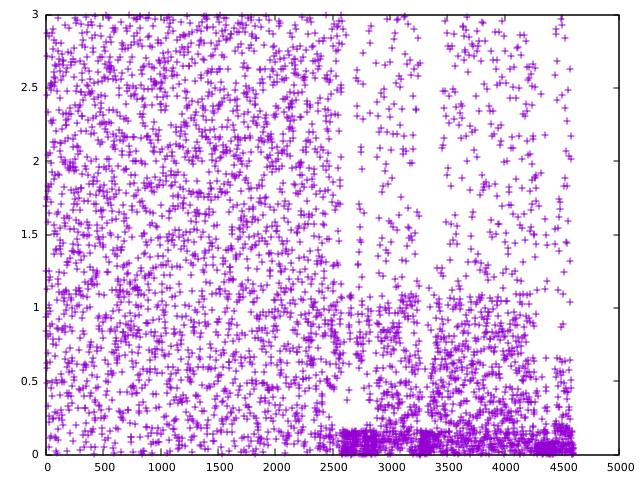
\includegraphics[width=0.5\textwidth]{adaptive_levi_dist.png}}
  \subfloat[График значения точек разбиения.]{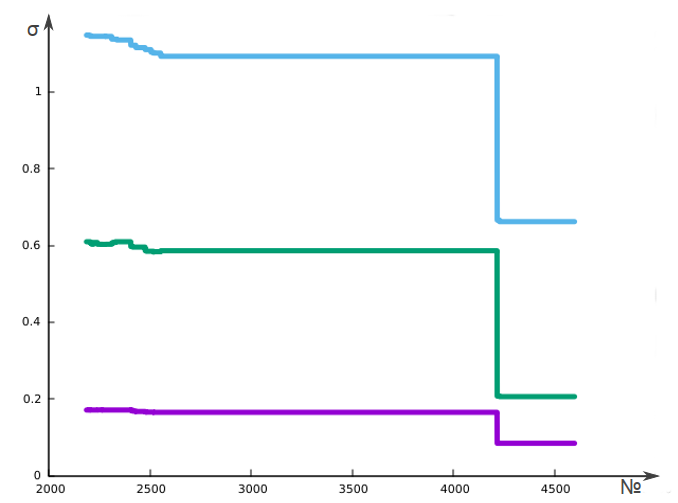
\includegraphics[width=0.5\textwidth]{adaptive_levi.png}}
  \caption{ Графики работы метода \textit{adaptive} для функции Леви.}
  \label{adaptive_levi_plot}
\end{figure}

\begin{figure}
  \centering
  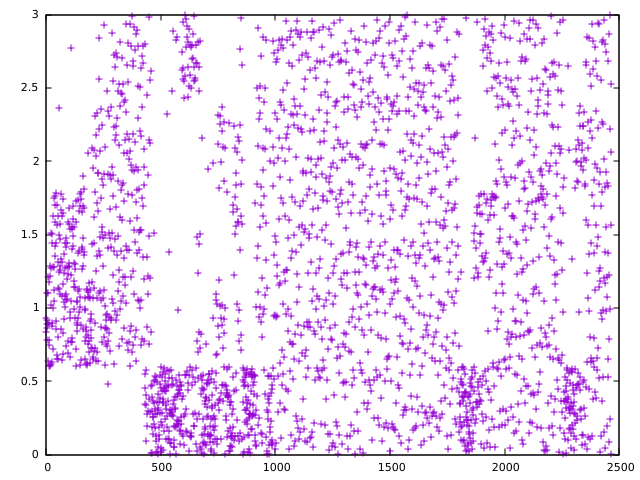
\includegraphics[width=0.5\textwidth]{karafotias_levi.png}
  \caption{График выбранных значений $\sigma$ в методе \textit{karafotias} для функции Леви.}
  \label{karafotias_levi}
\end{figure}

\section{Функция Растригина}

Леонард Растригин предложил нелинейную мультимодальную функцию для тестирования эффективности алгоритмов оптимизации. Нахождение минимума этой функции затруднено большим количеством локальных минимумов в области поиска. Функция задается формулой~(\ref{rastrigin_eq}).

\begin{equation}
\label{rastrigin_eq}
f(x_1, .., x_n) = An + \sum\limits_{i = 1}^n\left[ x_i^2 - Acos\left(2 \pi x_i \right)\right]
\end{equation}

\begin{figure}
    \centering
    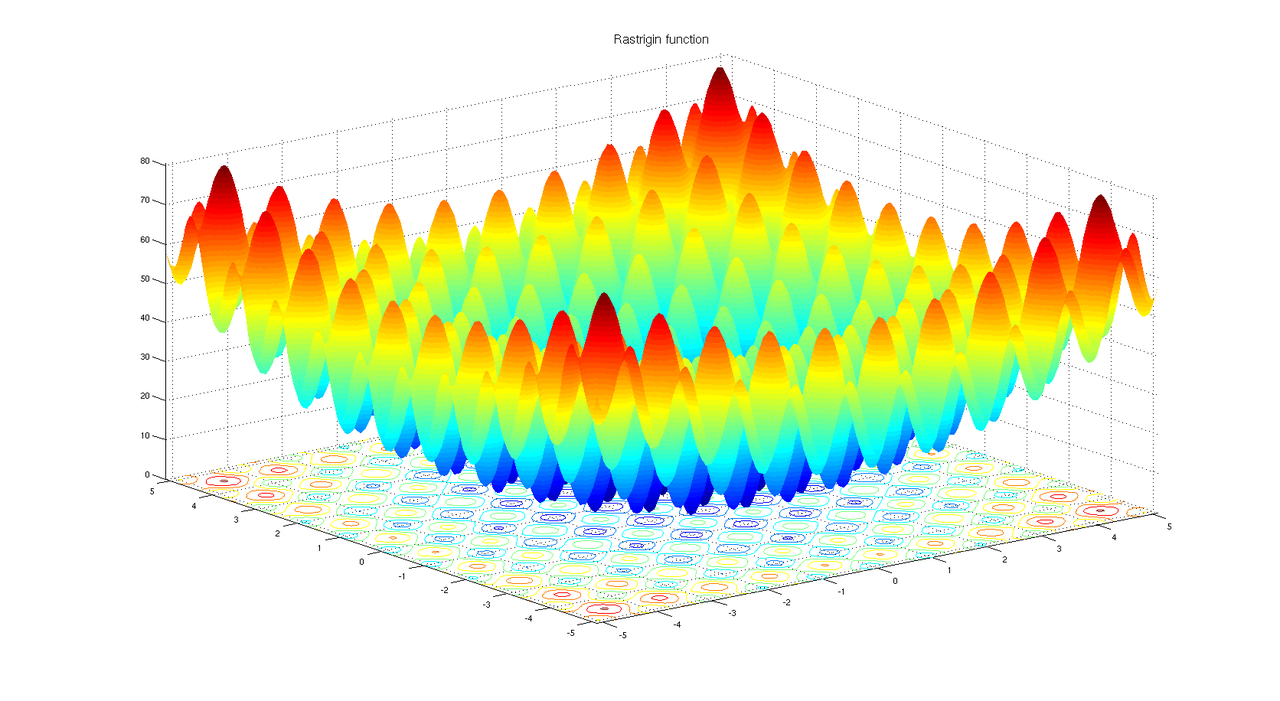
\includegraphics[width=0.6\textwidth]{rastrigin_2.png}
    \caption{График функции Растригина для двух переменных.}
    \label{rastrigin_plot}
\end{figure}

\begin{table}
  \centering
  \begin{tabular}{|*4{c|}}
  \hline
  \multicolumn{4}{|l|}{k = 1} \\
  \hline
  \diagbox{$\mu$}{$\lambda$} & \multicolumn{1}{c|}{1} & \multicolumn{1}{c|}{3} & \multicolumn{1}{c|}{7} \\
  \hline
  1& \cellcolor{olive}{5124} & \cellcolor{olive}{2301} & \cellcolor{olive}{1411} \\
  \hline
  5& \cellcolor{olive}{1859} & 1053 & \cellcolor{olive}{401} \\
  \hline
  10 & 1617 & 683 & 483 \\
  \hline
  \multicolumn{4}{|l|}{k = 2} \\
  \hline
  \diagbox{$\mu$}{$\lambda$} & \multicolumn{1}{c|}{1} & \multicolumn{1}{c|}{3} & \multicolumn{1}{c|}{7} \\
  \hline
  1& \cellcolor{olive}{5165} & \cellcolor{olive}{3461} & \cellcolor{olive}{1753} \\
  \hline
  5& \cellcolor{olive}{1990} & \cellcolor{olive}{1396} & \cellcolor{olive}{934} \\
  \hline
  10& \cellcolor{olive}{2022} & 1181 & 707 \\
  \hline
  \multicolumn{4}{|l|}{k = 3} \\
  \hline
  \diagbox{$\mu$}{$\lambda$} & \multicolumn{1}{c|}{1} & \multicolumn{1}{c|}{3} & \multicolumn{1}{c|}{7} \\
  \hline
  1& \cellcolor{olive}{6535}& \cellcolor{olive}{3391}& \cellcolor{olive}{2573} \\
  \hline
  5& \cellcolor{olive}{3148}& \cellcolor{olive}{1721}& \cellcolor{olive}{1231} \\
  \hline
  10& \cellcolor{olive}{2352} & 1677 & 1101 \\
  \hline
  \end{tabular}
  \captionsetup{justification=centering}
  \caption{Таблица с результатами применения метода \text{adaptive} для функции Растригина.}
\end{table}

\begin{table}
  \centering
  \begin{tabular}{|*7{c|}}
    \hline
    \multicolumn{7}{|l|}{k = 1} \\
    \hline
    \multirow{2}{*}{\diagbox{$\mu$}{$\lambda$}} & \multicolumn{2}{c|}{1} & \multicolumn{2}{c|}{3} & \multicolumn{2}{c|}{7} \\
    \cline{2-7}
    & q-learn & karafotias & q-learn & karafotias & q-learn & karafotias \\
    \hline
    1 & 15058 & 13418 & 3914 & 4167 & 1791 & 2330 \\
    \hline
    5 & 2311 & 2809 & 869& \cellcolor{olive}{748} & 533 & 665 \\
    \hline
    10 & \cellcolor{olive}{1497} & 1593& \cellcolor{olive}{488} & 616 & 290& \cellcolor{olive}{235} \\
    \hline
    \multicolumn{7}{|l|}{k = 2} \\
    \hline
    \multirow{2}{*}{\diagbox{$\mu$}{$\lambda$}} & \multicolumn{2}{c|}{1} & \multicolumn{2}{c|}{3} & \multicolumn{2}{c|}{7} \\
    \cline{2-7}
    & q-learn & karafotias & q-learn & karafotias & q-learn & karafotias \\
    \hline
    1 & 23371 & 27239 & 7295 & 7169 & 3488 & 2968 \\
    \hline
    5 & 8076 & 5810 & 2116 & 2705 & 1001 & 1247 \\
    \hline
    10 & 3415 & 2787& \cellcolor{olive}{1037} & 1106 & 811& \cellcolor{olive}{666} \\
    \hline
    \multicolumn{7}{|l|}{k = 3} \\
    \hline
    \multirow{2}{*}{\diagbox{$\mu$}{$\lambda$}} & \multicolumn{2}{c|}{1} & \multicolumn{2}{c|}{3} & \multicolumn{2}{c|}{7} \\
    \cline{2-7}
    & q-learn & karafotias & q-learn & karafotias & q-learn & karafotias \\
    \hline
    1 & 28702 & 36597 & 11427 & 9873 & 5820 & 6462 \\
    \hline
    5 & 12438 & 6791 & 2289 & 3673 & 1626 & 1255 \\
    \hline
    10 & 4473 & 6531 & 2000 & \cellcolor{olive}{1650} & 1137 & \cellcolor{olive}{1098} \\
    \hline
  \end{tabular}
  \captionsetup{justification=centering}
  \caption{Таблица с результатами применения методов \text{q-learn} и \text{karafotias} для функции Растригина.}
\end{table}

\begin{table}
  \centering
  \begin{tabular}{|*7{c|}}
    \hline
    \multicolumn{7}{|l|}{k = 1} \\
    \hline
    \multirow{2}{*}{\diagbox{$\mu$}{$\lambda$}} & \multicolumn{2}{c|}{1} & \multicolumn{2}{c|}{3} & \multicolumn{2}{c|}{7} \\
    \cline{2-7}
    & earpc & uearpc & earpc & uearpc & earpc & uearpc \\
    \hline
    1 & 9003 & 12905 & 3553& 2701 & 2296 & 1941 \\
    \hline
    5 & 5730 & 4453 & 1393 & 2749 & 1130 & 1258 \\
    \hline
    10 & 2213 & 3085 & 1161 & 1225 & 391 & 429 \\
    \hline
    \multicolumn{7}{|l|}{k = 2} \\
    \hline
    \multirow{2}{*}{\diagbox{$\mu$}{$\lambda$}} & \multicolumn{2}{c|}{1} & \multicolumn{2}{c|}{3} & \multicolumn{2}{c|}{7} \\
    \cline{2-7}
    & earpc & uearpc & earpc & uearpc & earpc & uearpc \\
    \hline
    1 & 20005 & 20819 & 7166 & 13342 & 5874 & 7870 \\
    \hline
    5 & 11153 & 11856 & 3775 & 4542 & 1775 & 2584 \\
    \hline
    10 & 8768 & 4603 & 3719 & 1648 & 1740 & 2558 \\
    \hline
    \multicolumn{7}{|l|}{k = 3} \\
    \hline
    \multirow{2}{*}{\diagbox{$\mu$}{$\lambda$}} & \multicolumn{2}{c|}{1} & \multicolumn{2}{c|}{3} & \multicolumn{2}{c|}{7} \\
    \cline{2-7}
    & earpc & uearpc & earpc & uearpc & earpc & uearpc \\
    \hline
    1 & 32533 & 43832 & 13061 & 10068 & 9797 & 9775 \\
    \hline
    5 & 8952 & 11581 & 4434 & 6799 & 3951 & 4914 \\
    \hline
    10 & 8320 & 10539 & 2611 & 2479 & 1742 & 1907 \\
    \hline
  \end{tabular}
  \captionsetup{justification=centering}
  \caption{Таблица с результатами применения методов \text{earpc} и \text{uearpc} для функции Растригина.}
\end{table}

\begin{figure}
  \centering
  \subfloat[График выбранных значений $\sigma$.]{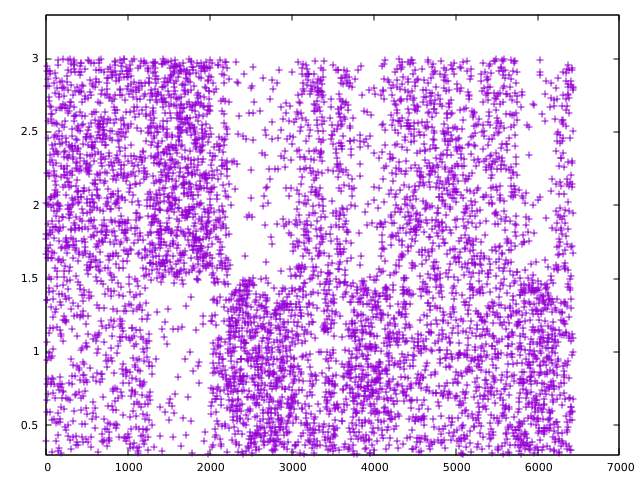
\includegraphics[width=0.5\textwidth]{earpc_rastrigin_dist.png}}
  \subfloat[График значения точки разбиения.]{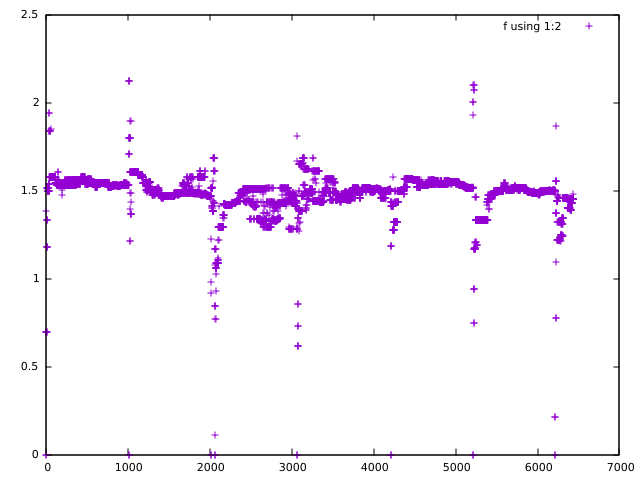
\includegraphics[width=0.5\textwidth]{earpc_rastrigin.png}}
  \caption{ Графики работы метода \textit{uarpc} для функции Растригина.}
  \label{uarpc_rastrigin_plot}
\end{figure}

\begin{figure}
  \centering
  \subfloat[График выбранных значений $\sigma$.]{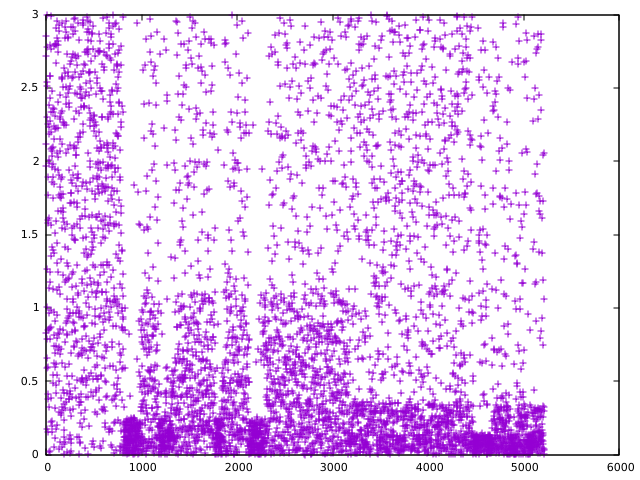
\includegraphics[width=0.5\textwidth]{adaptive_rastrigin_dist.png}}
  \subfloat[График значения точек разбиения.]{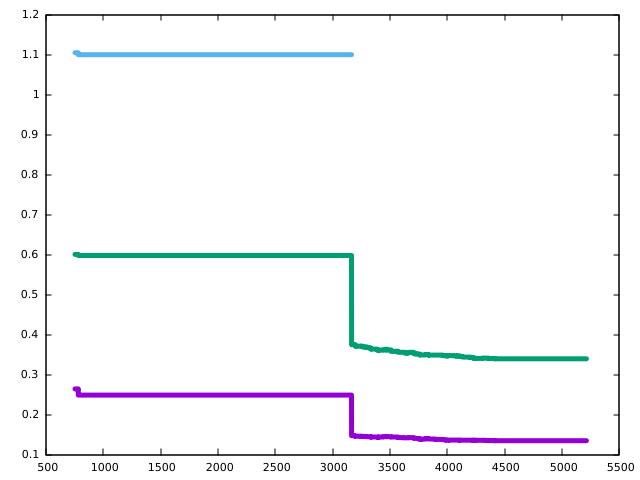
\includegraphics[width=0.5\textwidth]{adaptive_rastrigin.png}}
  \caption{ Графики работы метода \textit{adaptive} для функции Растригина.}
  \label{adaptive_rastrigin_plot}
\end{figure}

\begin{figure}
  \centering
  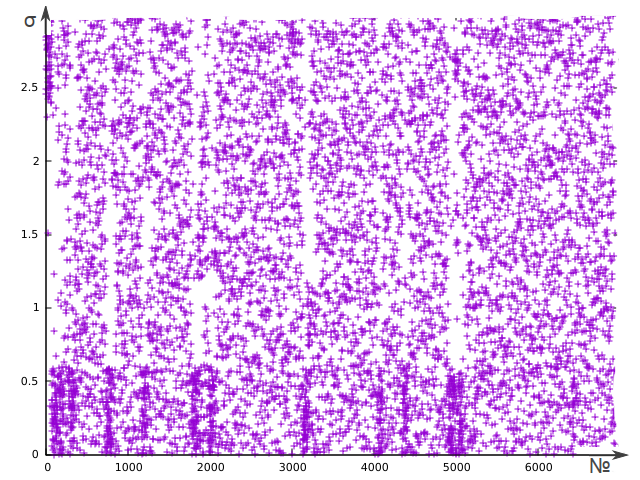
\includegraphics[width=0.5\textwidth]{karafotias_rastrigin.png}
  \caption{График выбранных значений $\sigma$ в методе \textit{karafotias} для функции Растригина.}
  \label{karafotias_rastrigin}
\end{figure}

\section{Выводы}

Методы адаптивной настройки параметров ЭА, предложенные в главе~\ref{proposed_chapter}, были протестированы на четырех модельных задачах. Было проведено сравнение предложенных методов с существующими алгоритмами настройки параметров ЭА. Наилучшие результаты были получены при использовании предложенного метода~(\ref{adaptive_method}). Было продемонстрировано, что данный метод улучшает значения настраеваемых параметров на протяжении всего процесса оптимизации в отличие от остальных рассмотренных методов.